\documentclass[../../labo_tp5_main.tex]{subfiles}

\begin{document}

%capítulo
\section{Ejercicio 7}
En Argentina, el espectro de frecuencias asignado a servicios de televisi\'on abarca desde los 54 MHz hasta los 806 MHZ, exceptuando la banda de 608 a 614 MHZ, que corresponde a Radioastronom\'ia. Est\'a dividido en canales desde el 2 hasta el 69. A cada canal le corresponden 6MHz. A su vez, est\'a divido en tres bandas:

\begin{table}[H]
\centering
\begin{tabular}{|c|c|}
\hline 
 & Canales \\ 
\hline 
BANDA I - VHF & 2 al 6 \\ 
\hline 
BANDA II - VHF & 7 al 13 \\ 
\hline 
BANDA  III - VHF & 21 al 69 ( menos 37) \\ 
\hline 
\end{tabular} 

\caption{Bandas del espectro destinado al servicio de televisi\'on}
\label{tab:TV_bandas}

\end{table}

Al igual que el espectro para FM, cada banda se divide en 4 categor\'ias seg\'un su radio de servicio, es decir hasta d\'onde la potencia de la estaci\'on se mantiene dentro de los 50$\frac{dB\mu}{m}$. En la tabla \ref{tab:tv_categoria_banda2} se muestra las categrias de la banda II, a la cual pertenece el canal sintonizado.

\begin{table}[H]
\centering
\begin{tabular}{|c|c|}
\hline 
CATEGOR\'IA & \begin{tabular}[c]{@{}l@{}}RADIO DE ÁREA ESTIMADA\\ (50 dB$\mu$ V/m - 316 $\mu$V/m)\\ Km.\end{tabular} \\ 
\hline 
PRINCIPAL & 75 \\ 
\hline 
SECUNDARIA & 55 \\ 
\hline 
MENOR & 40 \\ 
\hline 
LOCAL & 10 \\ 
\hline 
\end{tabular} 

\caption{Categor\'ias dentro de la banda II.}
\label{tab:tv_categoria_banda2}
\end{table}

El canal 11 tiene asignada la banda de frecuencias de 198 a 204 MHz. Se sintoniz\'o la portadora de audio a 203,85 MHz(tabla \ref{tab:canal11} y figura \ref{imagen})

\begin{table}[H]
\centering
\begin{tabular}{|l|l|}
\hline
Frecuencia & Contenido             \\ \hline
199,25     & Portadora de video    \\ \hline
202,83     & Subportadora de color \\ \hline
203,85     & Portadora de sonido   \\ \hline
\end{tabular}
\caption{Frecuencias de transmisi\'on del canal 11.}
\label{tab:canal11}
\end{table}

\begin{figure}[H]
	\centering
	\fbox{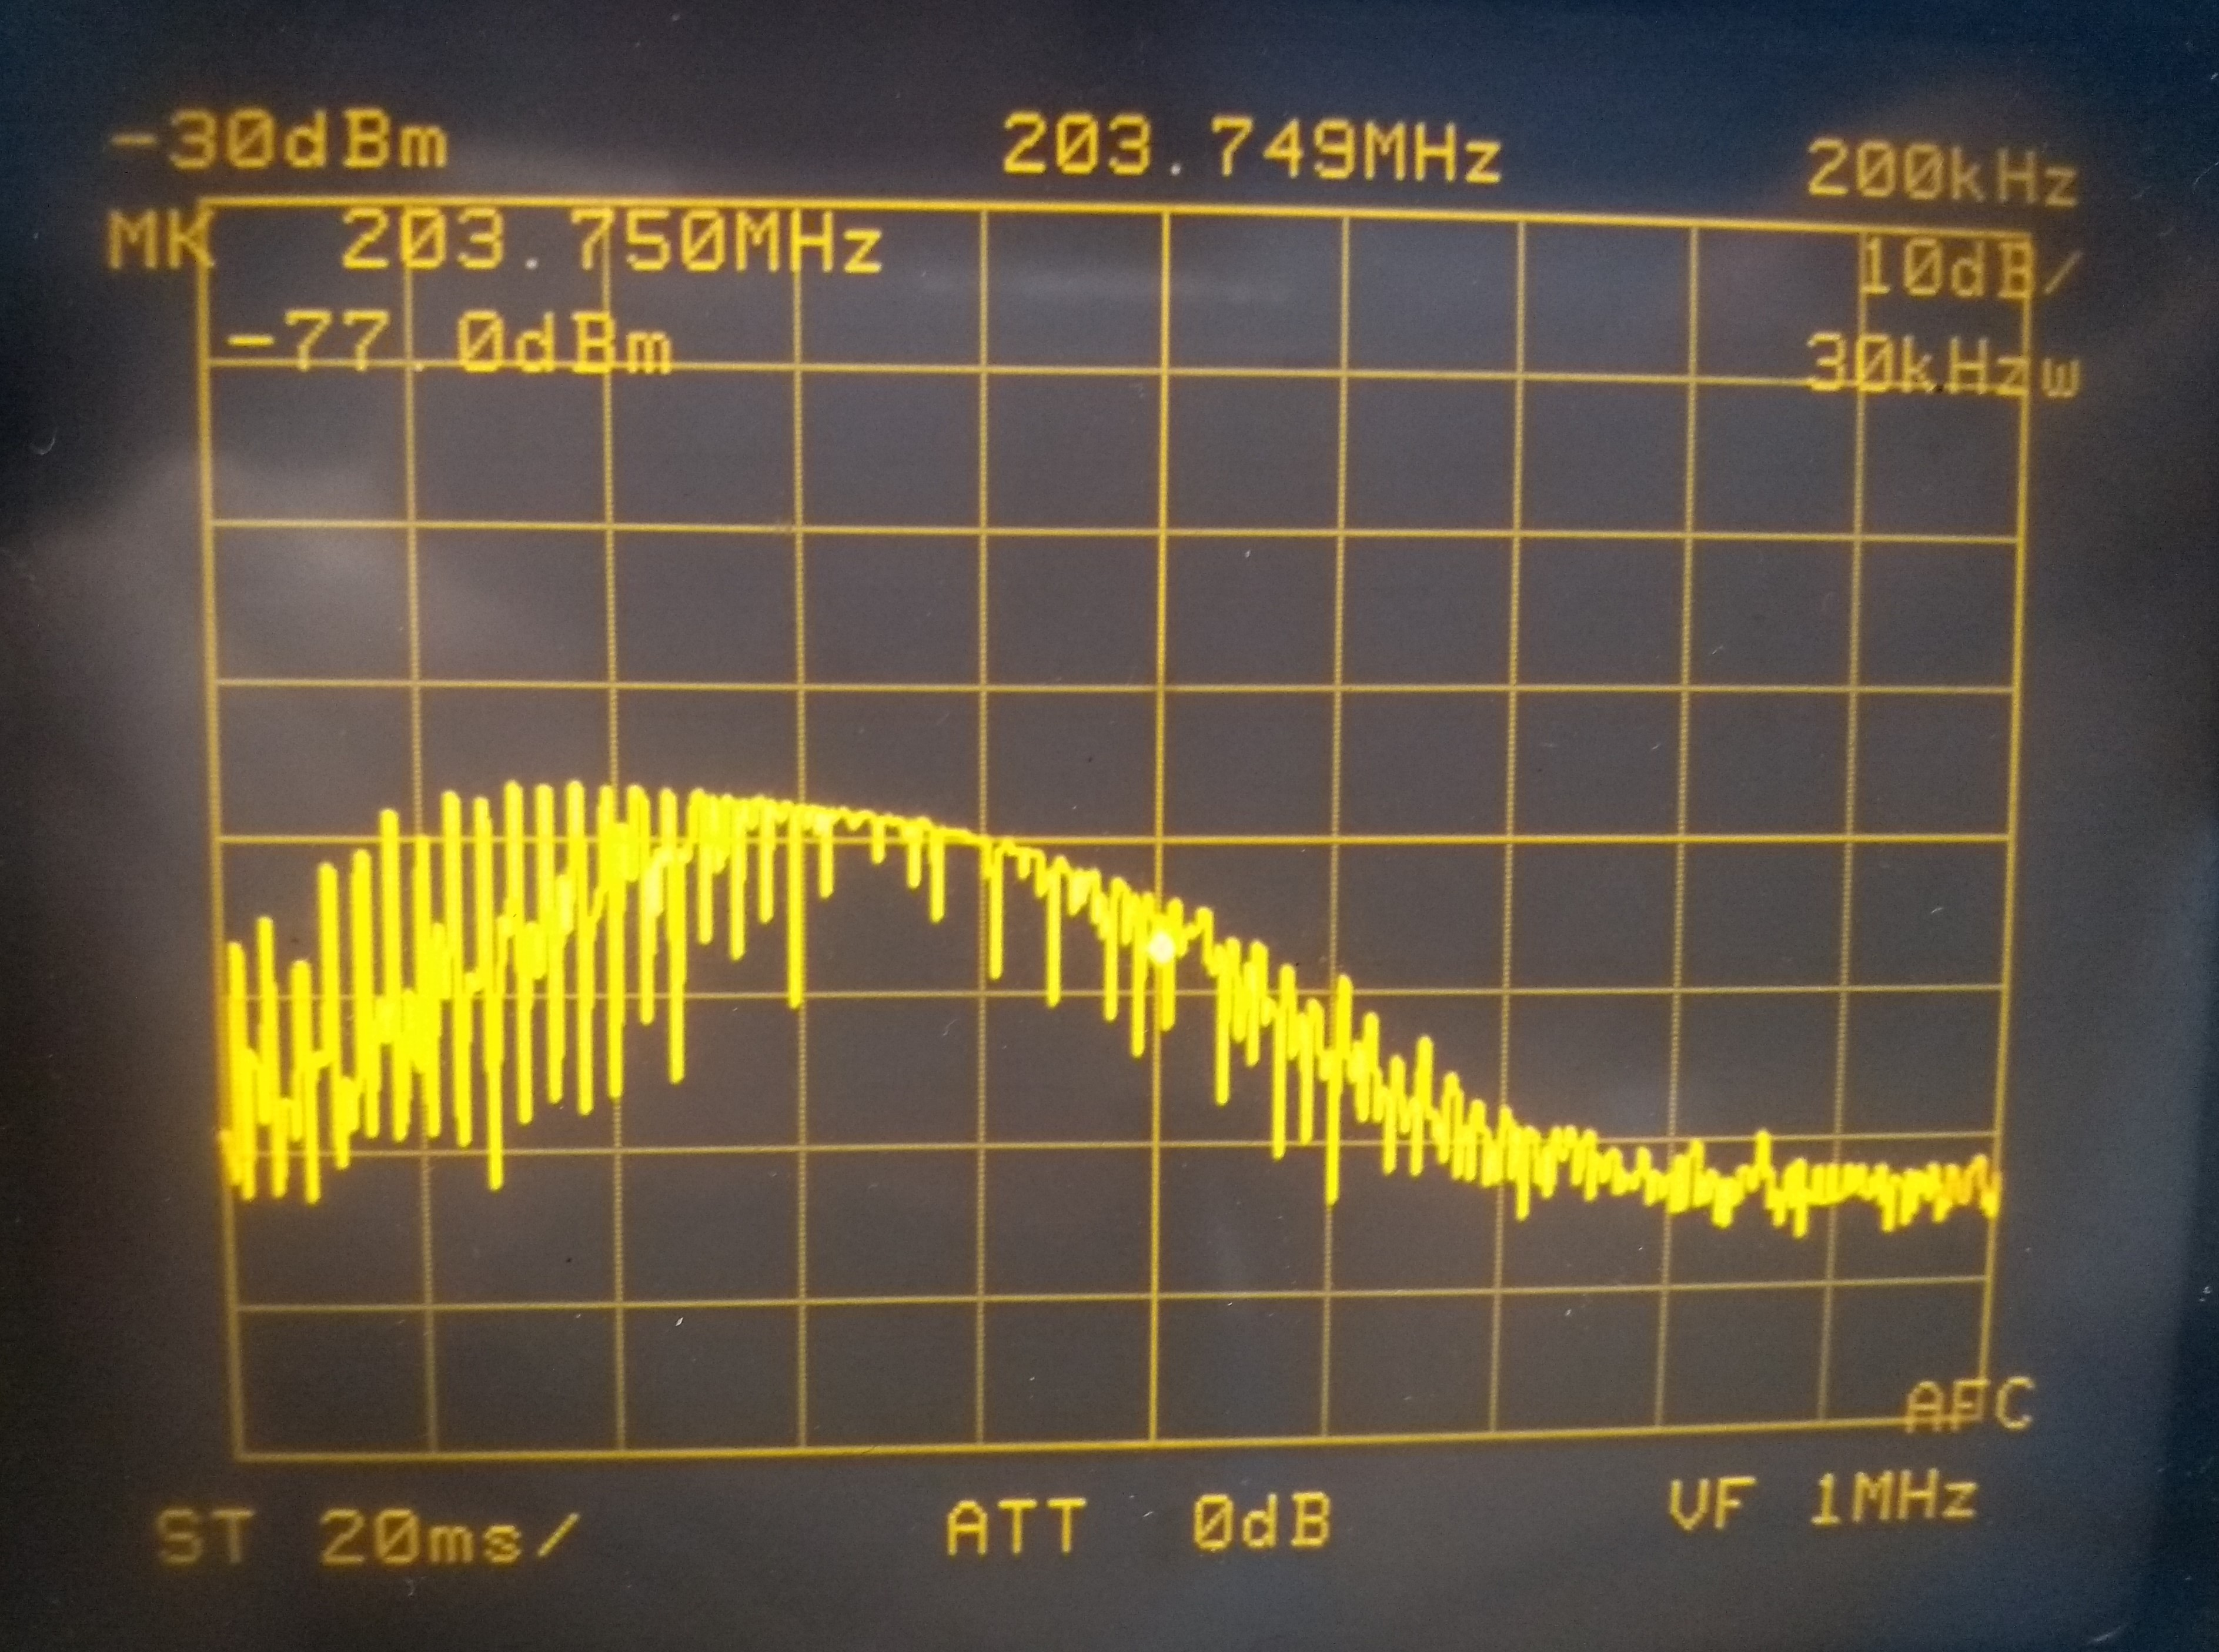
\includegraphics[scale=0.07]{imagenes/canal13.jpg}}
	\caption{Sintonizaci\'on a la radiodifusora canal 13.}
	\label{imagen}
\end{figure}





\end{document}
